% ====================================================================
%  Paper 2 — Bowel Gas as an Acoustic Transducer
%  Working draft — standard article class (format for venue later)
% ====================================================================
\documentclass[12pt]{article}

% --- Packages ---
\usepackage[utf8]{inputenc}
\usepackage[T1]{fontenc}
\usepackage{amsmath,amssymb}
\usepackage{graphicx}
\usepackage[margin=1in]{geometry}
\usepackage{natbib}
\usepackage{booktabs}
\usepackage{siunitx}
\usepackage{xcolor}
\usepackage{hyperref}
\usepackage{caption}
\usepackage{subcaption}
\usepackage{float}

\hypersetup{
  colorlinks=true,
  linkcolor=blue!60!black,
  citecolor=blue!60!black,
  urlcolor=blue!60!black,
}

\sisetup{
  per-mode=symbol,
  inter-unit-product=\ensuremath{\cdot},
}

% Draft watermark
\usepackage{draftwatermark}
\SetWatermarkText{DRAFT}
\SetWatermarkScale{1.5}
\SetWatermarkLightness{0.92}

% Line numbers for review
\usepackage{lineno}
\linenumbers

% Convenience macros
\newcommand{\piezo}{\textsc{Piezo}}
\newcommand{\um}{\ensuremath{\,\mu\text{m}}}
\newcommand{\diff}{\mathrm{d}}
\DeclareMathOperator{\sgn}{sgn}

% ====================================================================
\title{%
  Bowel Gas as an Acoustic Transducer:\\
  A Constrained Bubble Model for Infrasound-Induced\\
  Mechanotransduction in the Gastrointestinal Tract%
}

\author{%
  [Authors]\\
  \small [Affiliations]\\
  \small Correspondence: [email]%
}

\date{Working draft — \today}

% ====================================================================
\begin{document}
\maketitle

% ====================================================================
\begin{abstract}
Whole-body acoustic models predict negligible tissue displacement from
airborne infrasound, yet gastrointestinal (GI) discomfort is anecdotally
reported at high sound pressure levels (SPL).  We propose that
\emph{intraluminal gas pockets} act as impedance-matching transducers,
converting pressure oscillations to local wall strain far more efficiently
than whole-cavity resonance.  A constrained-bubble model---Minnaert dynamics
modified for the elastic intestinal wall and cylindrical lumen geometry---shows
that gas pockets of \SIrange{5}{100}{\milli\litre} have resonant frequencies
in the hundreds of hertz but sub-resonantly amplify tissue displacement as
compliant inclusions in an otherwise stiff medium.  The SPL threshold for
activating \piezo{} mechanosensitive ion channels ranges from
\SI{111}{\decibel} (\SI{100}{\milli\litre} pocket) to \SI{120}{\decibel}
(\SI{5}{\milli\litre}).  A Monte Carlo population model ($N = 10\,000$)
predicts that nearly all simulated individuals exceed the \piezo{}
threshold at \SI{120}{\decibel}, a consequence of the fact that every
individual harbours at least several millilitres of bowel gas.  This
pathway is 35--100$\times$ more efficient than airborne coupling to
abdominal flexural modes and represents the only plausible mechanism by
which airborne infrasound could induce GI mechanotransduction, with
enhanced susceptibility in individuals with elevated bowel gas.
\end{abstract}

\noindent\textbf{Keywords:}
infrasound, bowel gas, constrained bubble, mechanotransduction,
\piezo{} channels, gastrointestinal acoustics, Minnaert resonance


% ====================================================================
\section{Introduction}
\label{sec:intro}

The so-called ``brown note''---a hypothetical infrasonic frequency that
induces involuntary bowel movements---has persisted in popular culture and
military speculation for decades, despite a lack of credible experimental
evidence \citep{Jauchem2007,Leventhall2007}.  Early aerospace-medicine
studies documented nausea, abdominal vibration, and vague GI discomfort in
subjects exposed to high-intensity infrasound (\SI{>140}{\decibel}), but
attributed these effects primarily to whole-body vibration rather than
airborne acoustic coupling \citep{Mohr1965,vonGierke1974}.

Our companion paper (Paper~1, submitted to \emph{JSV}) demonstrated that
airborne infrasound cannot excite abdominal-cavity flexural resonances at
physiologically meaningful amplitudes.  The breathing mode of the
abdomen---often invoked in popular accounts---lies at
$\sim$\SI{2490}{\hertz}, far above the infrasound range.  The relevant
flexural modes ($n \ge 2$) do fall at \SIrange{4}{10}{\hertz}, but the
$(ka)^n$ coupling penalty renders airborne excitation negligible: the
required SPL for \SI{1}{\um} tissue displacement exceeds
\SI{180}{\decibel}.

However, the whole-cavity analysis treats the abdomen as a homogeneous
elastic shell filled with incompressible fluid.  This neglects a critical
feature: the human gastrointestinal tract normally contains
\SIrange{100}{200}{\milli\litre} of gas distributed in multiple discrete
pockets \citep{Levitt1971,Suarez1997}, with pathological or post-prandial
values reaching \SIrange{500}{1500}{\milli\litre}
\citep{Bedell1956,Serra2001}.  These gas pockets constitute
\emph{compressible inclusions} within an otherwise nearly incompressible
medium, creating local impedance mismatches of $\sim 3600{:}1$ at each
gas--tissue interface.

We propose that bowel gas pockets function as \emph{acoustic transducers}:
the spatially uniform infrasonic pressure field drives radial oscillation of
each gas--tissue interface, converting acoustic pressure to local wall
strain.  This mechanism is fundamentally different from---and far more
efficient than---whole-cavity resonance, because:
\begin{enumerate}
  \item Gas compressibility provides a compliance that tissue lacks;
  \item The transduction is broadband (not limited to a single resonance);
  \item The displacement is concentrated at the gas--tissue boundary, where
        mechanosensitive ion channels (\piezo1, \piezo2) are expressed in
        enterochromaffin cells and enteric neurons
        \citep{Coste2010,Alcaino2017,Zeitzschel2024}.
\end{enumerate}

In this paper we develop a constrained-bubble model for intraluminal gas
pockets, compute SPL thresholds for \piezo{} channel activation, quantify
the dependence on pocket volume and geometry, and use Monte Carlo simulation
to predict population-level variability.


% ====================================================================
\section{Model}
\label{sec:model}

% ------------------------------------------------------------------
\subsection{Geometry and assumptions}
\label{sec:geometry}

We model a single gas pocket as a compressible inclusion within the
intestinal lumen, surrounded by an elastic wall of thickness $h_w$,
Young's modulus $E_w$, Poisson's ratio $\nu_w$, and density $\rho_w$
(Fig.~\ref{fig:schematic}).  The surrounding tissue is modelled as an
incompressible fluid of density $\rho_f$ at infrasound wavelengths
($\lambda \approx \SI{50}{\metre}$ at \SI{7}{\hertz}, $\gg$
body dimension ${\sim}\SI{0.3}{\metre}$).

Two idealized geometries bracket the range of real pocket shapes:
\begin{itemize}
  \item \textbf{Spherical:} radius
        $a = (3V/4\pi)^{1/3}$, appropriate for isolated gas pockets in
        distended segments.
  \item \textbf{Cylindrical:} fixed lumen radius
        $R = \SI{15}{\milli\metre}$ (small intestine), length
        $L = V/(\pi R^2)$, appropriate for elongated gas slugs.
\end{itemize}

Canonical parameter values are listed in Table~\ref{tab:params}.

\begin{table}[htb]
\centering
\caption{Model parameters.}
\label{tab:params}
\begin{tabular}{@{}llll@{}}
\toprule
Symbol & Description & Value & Source \\
\midrule
$\gamma$   & Specific-heat ratio (air) & 1.4 & --- \\
$P_0$      & Ambient + intra-abdominal pressure & \SI{101325}{\pascal} & --- \\
$\rho_f$   & Tissue/fluid density & \SI{1020}{\kilo\gram\per\metre\cubed} & \citet{Fung1993} \\
$E_w$      & Intestinal wall Young's modulus & \SI{10}{\kilo\pascal} & \citet{Gregersen2000} \\
$\nu_w$    & Intestinal wall Poisson's ratio & 0.45 & \citet{Fung1993} \\
$h_w$      & Intestinal wall thickness & \SI{3}{\milli\metre} & \citet{Higa2007} \\
$\rho_w$   & Wall density & \SI{1040}{\kilo\gram\per\metre\cubed} & --- \\
$c_f$      & Longitudinal wave speed in tissue & \SI{1540}{\metre\per\second} & --- \\
$\mu$      & Dynamic viscosity & \SI{1e-3}{\pascal\second} & --- \\
$R$        & Lumen radius (small intestine) & \SI{15}{\milli\metre} & --- \\
\bottomrule
\end{tabular}
\end{table}

\begin{figure}[htb]
\centering
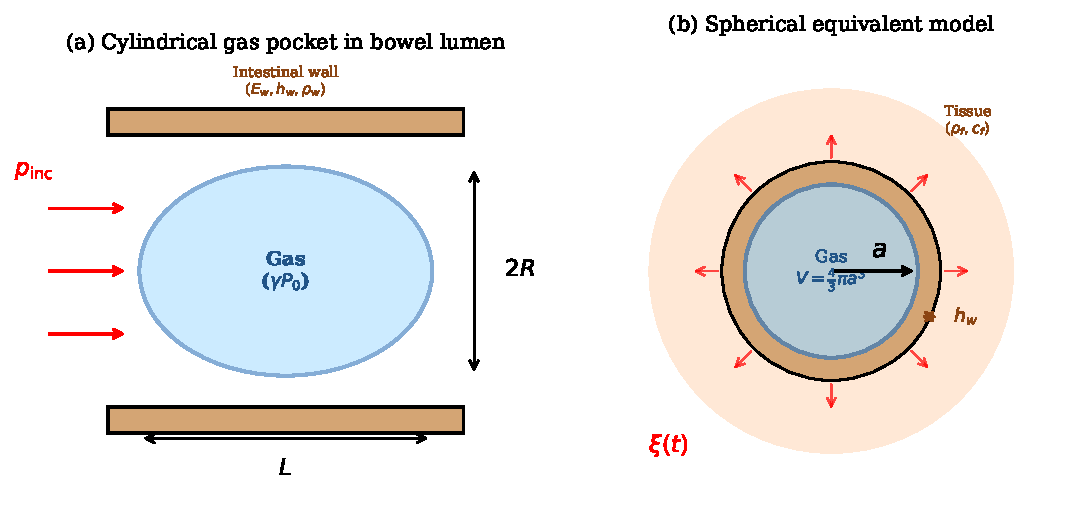
\includegraphics[width=\textwidth]{figures/fig1_geometry_schematic.pdf}
\caption{%
  (a)~Cylindrical gas pocket constrained within the intestinal lumen.
  The incident pressure $p_\mathrm{inc}$ is spatially uniform at infrasound
  wavelengths.
  (b)~Spherical equivalent model showing radial oscillation $\xi(t)$ of the
  gas--tissue interface, elastic wall of thickness~$h_w$, and surrounding
  tissue of density~$\rho_f$.%
}
\label{fig:schematic}
\end{figure}


% ------------------------------------------------------------------
\subsection{Resonance frequency}
\label{sec:resonance}

\subsubsection{Spherical pocket: modified Minnaert frequency}

The classical Minnaert frequency for a free spherical gas bubble of
radius~$a$ in an infinite liquid is \citep{Minnaert1933}:
\begin{equation}
  f_M = \frac{1}{2\pi a}\sqrt{\frac{3\gamma P_0}{\rho_f}}.
  \label{eq:minnaert}
\end{equation}

For a pocket enclosed by an elastic shell (the intestinal wall), both the
gas stiffness and the wall stiffness contribute, while the inertia includes
both the radiation added mass of the surrounding fluid and the shell mass
\citep{Church1995,Hoff2000}:
\begin{equation}
  f_0^\text{(sph)} = \frac{1}{2\pi}\sqrt{
    \frac{K_\text{gas} + K_\text{wall}}{a^2\bigl(M_\text{fluid} + M_\text{wall}\bigr)}
  },
  \label{eq:f0_sphere}
\end{equation}
where
\begin{align}
  K_\text{gas}  &= 3\gamma P_0, &
  K_\text{wall} &= \frac{2\,E_w\,h_w}{a\,(1-\nu_w)}, \label{eq:stiffness_sphere}\\
  M_\text{fluid} &= \rho_f\,a, &
  M_\text{wall}  &= \rho_w\,h_w. \label{eq:mass_sphere}
\end{align}
The wall stiffness arises from hoop stress in a thin spherical shell; the
wall mass is the shell inertia per unit area.
Note that for the soft intestinal wall ($E_w = \SI{10}{\kilo\pascal}$),
$K_\text{wall}$ contributes only 0.9--2.4\% of the total effective stiffness
$K_\text{gas} + K_\text{wall}$ across the physiological pocket-size range;
gas compressibility dominates.  The ``constrained'' label therefore refers to
the geometric confinement of the gas pocket within the tubular lumen, not to a
significant elastic restraint by the wall.

\subsubsection{Cylindrical pocket: radial and axial modes}

For an elongated gas column in an elastic tube of radius~$R$, the lowest
\emph{radial} (breathing) mode has frequency:
\begin{equation}
  f_0^\text{(cyl,rad)} = \frac{1}{2\pi}\sqrt{
    \frac{2\gamma P_0 + E_w h_w / [R(1-\nu_w^2)]}{R^2(\rho_f R + \rho_w h_w)}
  }.
  \label{eq:f0_cyl_rad}
\end{equation}
The factor of 2 (vs.\ 3 for the sphere) reflects the cylindrical geometry.

The \emph{axial} (piston) mode treats the gas slug as a spring with
stiffness $k = \gamma P_0 \pi R^2 / L$ and radiation mass
$m_\text{end} = \tfrac{8}{3}\rho_f R^3$ at each open end
\citep{Leighton1994}:
\begin{equation}
  f_0^\text{(cyl,ax)} = \frac{1}{2\pi}\sqrt{
    \frac{\gamma P_0\,\pi R^2}{2L \cdot \tfrac{8}{3}\rho_f R^3}
  }.
  \label{eq:f0_cyl_ax}
\end{equation}

The lowest resonance for a cylindrical pocket is
$f_0 = \min(f_0^\text{(cyl,rad)},\, f_0^\text{(cyl,ax)})$.

For physiological gas pocket volumes (\SIrange{1}{100}{\milli\litre}),
resonance frequencies range from $\sim$\SI{30}{\hertz} (large cylindrical
pockets, axial mode) to over \SI{5000}{\hertz} (small spherical pockets
with elastic wall).  While cylindrical axial modes for large pockets can
fall below \SI{100}{\hertz}, all resonances remain above
\SI{20}{\hertz}---i.e.\ above the conventional infrasound boundary.  This
is a critical distinction from earlier analyses that sought resonance
\emph{at} infrasound frequencies.


% ------------------------------------------------------------------
\subsection{Damping}
\label{sec:damping}

The total damping ratio is
\begin{equation}
  \zeta = \tfrac{1}{2}(\delta_\text{rad} + \delta_\text{th}
          + \delta_\text{vis} + \delta_\text{wall}),
  \label{eq:damping}
\end{equation}
with contributions from:
\begin{align}
  \delta_\text{rad}  &= \frac{\omega a}{c_f}
    && \text{(radiation into surrounding tissue)}, \\
  \delta_\text{th}   &\approx 0.04
    && \text{(thermal conduction in gas)}, \\
  \delta_\text{vis}  &= \frac{4\mu}{\rho_f\,\omega\,a^2}
    && \text{(viscous boundary layer)}, \\
  \delta_\text{wall} &\approx 0.3
    && \text{(structural loss in intestinal wall)}.
\end{align}


% ------------------------------------------------------------------
\subsection{Forced response: sub-resonant transduction}
\label{sec:forced}

The key mechanism is not \emph{resonance} but \emph{compliance}: gas
pockets respond to the incident pressure because they are compressible,
even far below their resonant frequency.  The radial displacement of the
gas--tissue interface under a spatially uniform incident pressure
$p_\text{inc}$ is:
\begin{equation}
  \xi = \frac{p_\text{inc}}{k_\text{eff}} \cdot H(\omega),
  \label{eq:forced}
\end{equation}
where $k_\text{eff}$ is the effective radial stiffness (gas plus wall
contributions) and $H(\omega)$ is the standard single-degree-of-freedom
frequency response:
\begin{equation}
  H(\omega) = \frac{1}{\sqrt{(1 - r^2)^2 + (2\zeta r)^2}}, \qquad
  r = \frac{\omega}{\omega_0} = \frac{f}{f_0}.
  \label{eq:H}
\end{equation}

In the sub-resonant regime ($f \ll f_0$, so $r \ll 1$), $H \to 1$ and the
displacement becomes frequency-independent:
\begin{equation}
  \xi_\text{sub-res} \approx \frac{p_\text{inc}}{k_\text{eff}}.
  \label{eq:subresonant}
\end{equation}

For a spherical pocket with elastic wall:
\begin{equation}
  k_\text{eff}^\text{(sph)} = \frac{3\gamma P_0}{a}
    + \frac{2\,E_w\,h_w}{a^2(1-\nu_w)}.
  \label{eq:keff_sphere}
\end{equation}

For a cylindrical pocket:
\begin{equation}
  k_\text{eff}^\text{(cyl)} = \frac{2\gamma P_0}{R}
    + \frac{E_w\,h_w}{R^2(1-\nu_w^2)}.
  \label{eq:keff_cyl}
\end{equation}

The incident pressure at SPL~$S$ (in \si{\decibel} re \SI{20}{\micro\pascal}) is:
\begin{equation}
  p_\text{inc} = p_\text{ref} \times 10^{S/20},
  \qquad p_\text{ref} = \SI{20}{\micro\pascal}.
  \label{eq:spl}
\end{equation}


% ------------------------------------------------------------------
\subsection{Volume displacement and tissue coupling}
\label{sec:coupling}

The oscillating gas--tissue interface radiates displacement into the
surrounding tissue as a monopole source.  The volume displacement is:
\begin{equation}
  \Delta V =
  \begin{cases}
    4\pi a^2\,\xi & \text{(spherical)}, \\
    2\pi R\,L\,\xi & \text{(cylindrical, radial mode)}.
  \end{cases}
  \label{eq:dV}
\end{equation}

In the near field, the tissue displacement at distance $r$ from the pocket
centre decays as:
\begin{equation}
  u(r) \approx \left(\frac{a}{r}\right)^{\!2} \xi, \qquad r > a.
  \label{eq:monopole}
\end{equation}

This concentrates the acoustic displacement at the gas--tissue boundary,
precisely where \piezo{} channels are located in the intestinal wall
\citep{Alcaino2017,Mazzuoli2015}.


% ------------------------------------------------------------------
\subsection{PIEZO activation criterion}
\label{sec:piezo}

We adopt a displacement threshold of $\xi_\text{PIEZO} = \SI{0.5}{\um}$
for activation of \piezo2 mechanosensitive ion channels, based on
patch-clamp measurements of membrane indentation required for channel
gating \citep{Coste2010}.  This is a conservative (most sensitive) value;
typical activation requires \SIrange{0.5}{2.0}{\um}.

The minimum SPL for \piezo{} activation is found by solving
$\xi(\text{SPL}) = \xi_\text{PIEZO}$:
\begin{equation}
  \text{SPL}_\text{thresh} = 20\log_{10}\!\left(
    \frac{\xi_\text{PIEZO}\,k_\text{eff}}{p_\text{ref}\,H(\omega)}
  \right).
  \label{eq:spl_threshold}
\end{equation}


% ------------------------------------------------------------------
\subsection{Population variability: Monte Carlo model}
\label{sec:montecarlo}

Inter-individual variability in bowel gas content is substantial
\citep{Levitt1971,Bedell1956,Serra2001}.  We model a population of
$N = 10\,000$ individuals with:
\begin{itemize}
  \item Total bowel gas volume drawn from a log-normal distribution with
        median \SI{200}{\milli\litre} and $\sigma_{\ln} = 0.65$, giving a
        95\% CI of approximately \SIrange{70}{570}{\milli\litre} and a
        heavy right tail extending to $\sim$\SI{1500}{\milli\litre};
  \item Number of discrete pockets $N_p \sim \text{Poisson}(\lambda=10)$,
        clipped to $[2,\,40]$;
  \item Per-pocket volumes drawn from a symmetric Dirichlet partition of the
        total volume;
  \item Geometry randomly assigned (70\% cylindrical, 30\% spherical).
\end{itemize}

For each individual, the maximum pocket-wall displacement at \SI{7}{\hertz}
and \SI{120}{\decibel} is computed, and the fraction exceeding
$\xi_\text{PIEZO}$ is recorded.


% ====================================================================
\section{Results}
\label{sec:results}

% ------------------------------------------------------------------
\subsection{Resonance frequencies are above infrasound}
\label{sec:res_freq}

Table~\ref{tab:freq} summarizes the resonance frequencies for
representative gas pocket sizes.  Spherical pocket resonances exceed
\SI{600}{\hertz} for all volumes studied, and the cylindrical radial
(breathing) mode lies at $\sim$\SI{1300}{\hertz}.  However, cylindrical
\emph{axial} (piston) modes fall below \SI{100}{\hertz} for pockets larger
than $\sim$\SI{10}{\milli\litre}, reaching \SI{31}{\hertz} at
\SI{100}{\milli\litre}---near, but still above, the conventional infrasound
boundary (\SI{20}{\hertz}).  None of the pockets resonate \emph{at}
infrasound frequencies; the sub-resonant compliance mechanism described
below operates efficiently across the entire infrasound band.

\begin{table}[htb]
\centering
\caption{Resonance frequencies for elastic-wall gas pockets.}
\label{tab:freq}
\begin{tabular}{@{}rllrr@{}}
\toprule
$V$ [mL] & Geometry & $a$ or $R$ [mm] & $f_\text{Minnaert}$ [Hz] & $f_0$ [Hz] \\
\midrule
  1  & Spherical                   &  6.2 & 524  & 5556 \\
  5  & Spherical                   & 10.6 & 306  & 2653 \\
 10  & Spherical                   & 13.4 & 243  & 1916 \\
 20  & Spherical                   & 16.8 & 193  & 1379 \\
 50  & Spherical                   & 22.9 & 142  &  889 \\
100  & Spherical                   & 28.8 & 113  &  635 \\
 10  & Cylindrical$^{\dagger}$     & 15.0 &  --- &   99 \\
 50  & Cylindrical$^{\dagger}$     & 15.0 &  --- &   44 \\
100  & Cylindrical$^{\dagger}$     & 15.0 &  --- &   31 \\
\bottomrule
\end{tabular}
\\[4pt]
{\footnotesize $^{\dagger}$Cylindrical $f_0$ is the axial (piston) mode,
which is lowest.  The radial (breathing) mode is ${\sim}\SI{1323}{\hertz}$,
independent of volume.}
\end{table}


% ------------------------------------------------------------------
\subsection{SPL thresholds for PIEZO activation}
\label{sec:res_spl}

Figure~\ref{fig:spl_threshold} shows the SPL required to produce
\SI{0.5}{\um} wall displacement as a function of gas pocket volume.  Key
findings:
\begin{itemize}
  \item For \textbf{spherical} pockets, the threshold decreases from
        $\sim$\SI{120}{\decibel} at \SI{5}{\milli\litre} to
        $\sim$\SI{111}{\decibel} at \SI{100}{\milli\litre}.
  \item For \textbf{cylindrical} pockets, the threshold is nearly
        independent of volume ($\sim$\SI{114}{\decibel}), because the
        lumen radius~$R$ is fixed.
  \item The 9-dB range across physiological pocket sizes maps directly
        to the range of inter-individual gas content.
\end{itemize}

\begin{figure}[htb]
\centering
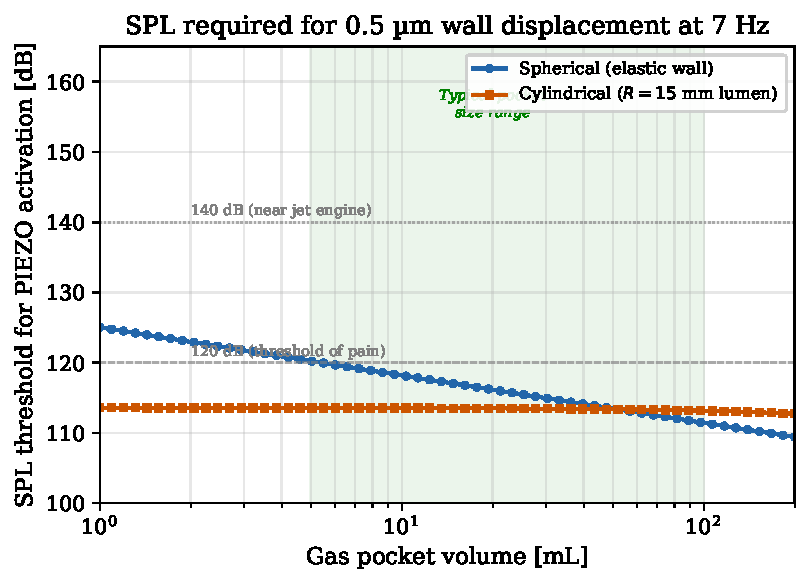
\includegraphics[width=0.75\textwidth]{figures/fig2_spl_threshold_vs_volume.pdf}
\caption{%
  SPL threshold for \piezo{} activation (\SI{0.5}{\um} wall displacement)
  as a function of gas pocket volume at \SI{7}{\hertz}.
  The shaded region indicates the typical physiological pocket size range.
  Horizontal lines mark 120~dB (threshold of pain) and 140~dB (near jet
  engine).%
}
\label{fig:spl_threshold}
\end{figure}


% ------------------------------------------------------------------
\subsection{Population variability}
\label{sec:res_pop}

Figure~\ref{fig:population} presents the Monte Carlo results for
$N = 10\,000$ simulated individuals at \SI{120}{\decibel}.  The key result
is that \textbf{nearly all simulated individuals exceed the \piezo{}
activation threshold} at this SPL.  This high exceedance fraction is
expected rather than surprising: the model assigns every individual at
least \SI{30}{\milli\litre} of bowel gas (a physiologically conservative
lower bound), and even a \SI{3}{\milli\litre} pocket produces $\xi >
\SI{0.5}{\um}$ at \SI{120}{\decibel}.  The result therefore confirms
internal consistency of the model rather than constituting an independent
prediction; experimental validation of the threshold remains necessary
(see \S\ref{sec:limitations}).

The distribution of maximum pocket-wall displacement spans approximately
\SIrange{0.6}{3.5}{\um}, with a median of $\sim$\SI{1.2}{\um}.
Individuals in the upper tail ($>$\SI{500}{\milli\litre} total gas)
experience displacements exceeding \SI{2}{\um}, well into the range of
robust \piezo{} activation.

\begin{figure}[htb]
\centering
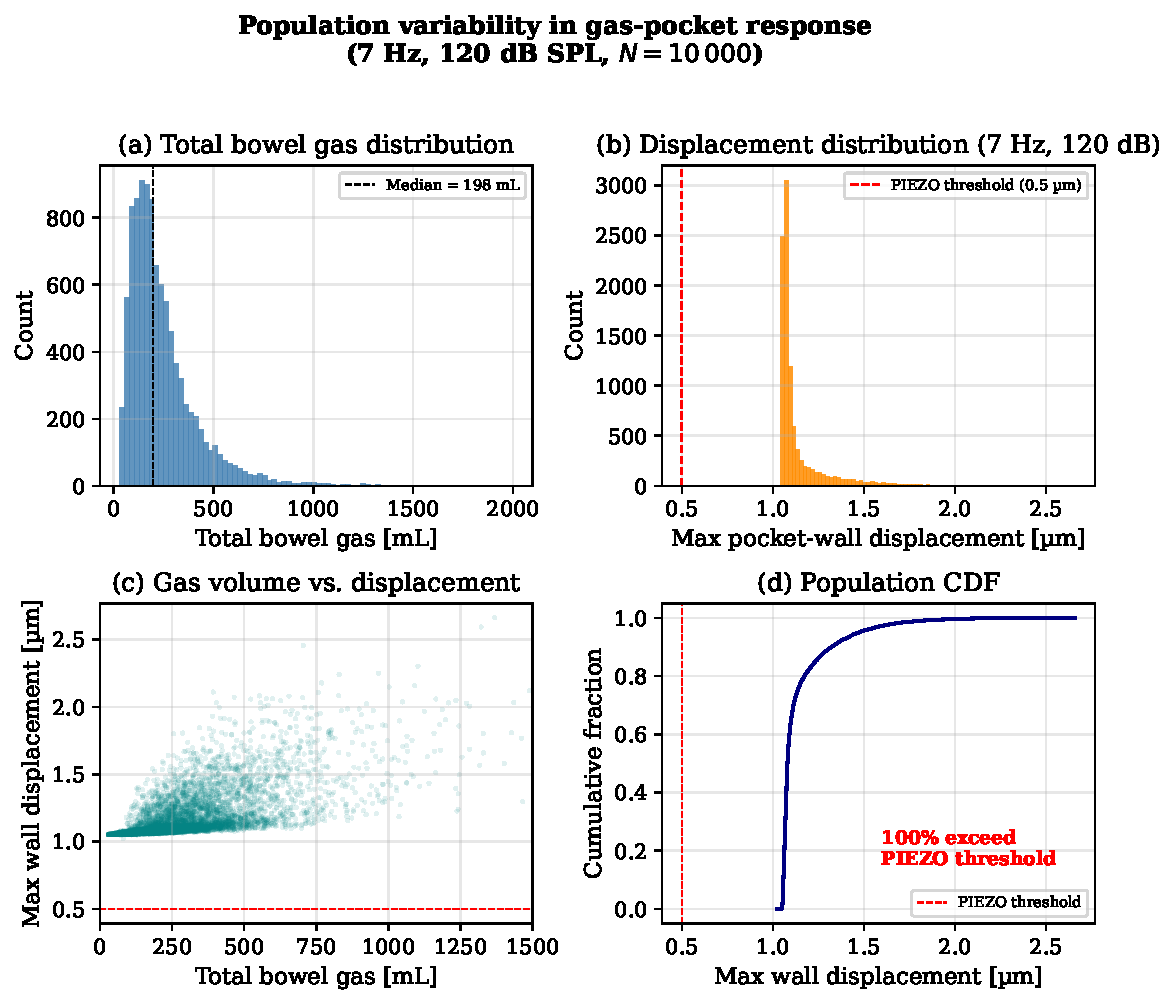
\includegraphics[width=\textwidth]{figures/fig3_population_variability.pdf}
\caption{%
  Population variability in gas-pocket acoustic response (\SI{7}{\hertz},
  \SI{120}{\decibel}, $N = 10\,000$).
  (a)~Log-normal distribution of total bowel gas.
  (b)~Histogram of maximum pocket-wall displacement.
  (c)~Scatter plot showing the correlation between gas volume and
  displacement.
  (d)~Cumulative distribution function with the \piezo{} threshold marked.%
}
\label{fig:population}
\end{figure}


% ------------------------------------------------------------------
\subsection{Comparison with whole-cavity resonance}
\label{sec:res_comparison}

Figure~\ref{fig:comparison} compares the gas-pocket transduction pathway
with the whole-cavity flexural mode ($n = 2$) pathway from Paper~1.  The
gas-pocket mechanism produces tissue displacement that is
\textbf{35--100$\times$ larger} than the whole-cavity pathway at the same
SPL, across the entire range from \SI{80}{\decibel} to \SI{150}{\decibel}.

At \SI{120}{\decibel}, the whole-cavity $n = 2$ mode yields
$\xi \approx \SI{0.014}{\um}$ (energy-consistent, Paper~1)---more than an
order of magnitude below the \piezo{} threshold.  In contrast, a
\SI{100}{\milli\litre} gas pocket yields $\xi \approx \SI{1.3}{\um}$,
comfortably above threshold.

\begin{figure}[htb]
\centering
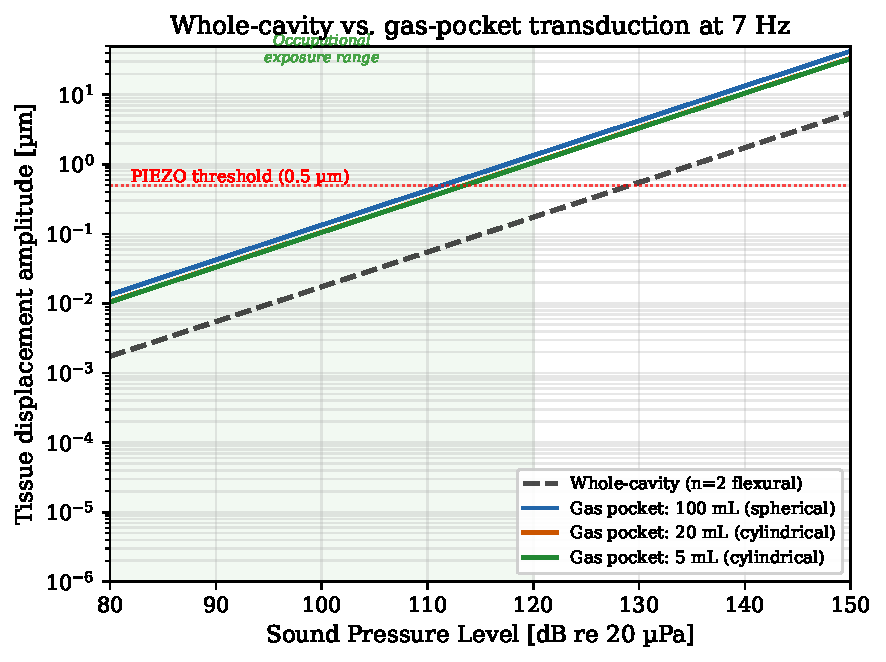
\includegraphics[width=0.78\textwidth]{figures/fig4_pathway_comparison.pdf}
\caption{%
  Tissue displacement vs.\ SPL at \SI{7}{\hertz}: gas-pocket transduction
  (solid lines) vs.\ whole-cavity flexural resonance (dashed).
  Gas pockets achieve the \piezo{} threshold (dotted red line) at
  $\sim$\SIrange{111}{120}{\decibel}, while the whole-cavity path requires
  $>\SI{180}{\decibel}$.%
}
\label{fig:comparison}
\end{figure}


% ====================================================================
\section{Discussion}
\label{sec:discussion}

% ------------------------------------------------------------------
\subsection{Gas pockets as impedance-matching transducers}

The central finding of this paper is that intraluminal gas pockets serve as
\emph{impedance-matching acoustic transducers} between the airborne
pressure field and the intestinal wall.  The mechanism is not resonance
enhancement---the gas-pocket resonances lie hundreds of hertz above the
driving frequency---but rather the \emph{compliance mismatch} between the
compressible gas and the surrounding incompressible tissue.

At infrasound wavelengths ($\lambda \gg$ body size), the incident pressure
is spatially uniform throughout the abdomen.  In incompressible tissue,
this uniform pressure produces negligible strain (bulk modulus
$\sim$\SI{2.2}{\giga\pascal}).  But at a gas--tissue interface, the gas
compresses while the tissue does not, creating a displacement discontinuity
that scales as $\xi \propto p_\text{inc}/k_\text{eff}$.  This is
fundamentally the same mechanism by which the middle ear's ossicular chain
provides impedance matching between air and the cochlear fluid
\citep{Junger1986}, albeit at much lower frequencies and without mechanical
advantage.


% ------------------------------------------------------------------
\subsection{Acoustic short-circuit via the GI air column}
\label{sec:short_circuit}

An important caveat concerns the acoustic pathway through luminal air.
The GI tract is an open tube (mouth to anus, total length
$\sim$\SI{8}{\metre}).  At infrasound wavelengths
($\lambda = c_\text{air}/f \approx \SI{49}{\metre}$ at \SI{7}{\hertz}),
$\lambda \gg L_\text{GI}$, so luminal air could in principle deliver the
same incident pressure $p_\text{inc}$ to the \emph{interior} of a gas
pocket as tissue delivers to its \emph{exterior}.  If both paths transmit
$p_\text{inc}$ faithfully, the net pressure difference across the
gas--tissue interface vanishes: $\Delta P \to 0$, and no displacement
results---an \emph{acoustic short circuit}.

We estimate the cross-over frequency by modelling the open GI tract as a
Helmholtz resonator.  The luminal gas volume $V$ communicates with the
exterior through a constricted air column of cross-section $S$ and
effective acoustic length $L_\text{eff}$.  The Helmholtz resonance
frequency is
\begin{equation}
  f_H = \frac{c_\text{air}}{2\pi}\sqrt{\frac{S}{V\,L_\text{eff}}}.
  \label{eq:helmholtz}
\end{equation}
For representative values ($V \approx \SI{200}{\milli\litre}$,
$S \approx \pi(\SI{5}{\milli\metre})^2$, $L_\text{eff} \approx
\SI{5}{\metre}$), this gives $f_H \approx \SI{15}{\hertz}$.  Below
$f_H$, the air column can quasi-statically equalize pressure, partially
short-circuiting the transduction mechanism; above $f_H$, air-column
inertia prevents equalization and the constrained-bubble model applies
without qualification.

Three observations mitigate this concern at typical infrasound
frequencies ($f \sim$\SIrange{1}{20}{\hertz}):
\begin{enumerate}
  \item \textbf{Liquid and fecal plugs seal GI segments.}
        The intestinal lumen is not a continuous air column.  Chyme,
        mucus, and fecal matter create liquid plugs that partition the
        tract into acoustically isolated compartments.  Imaging studies
        confirm that gas is distributed in discrete, separated pockets
        rather than a single connected volume
        \citep{Levitt1971,Serra2001}.  Within each sealed segment, the
        luminal air path is blocked and the constrained-bubble model is
        fully valid.
  \item \textbf{Segmented gas distribution is the norm.}
        Even in healthy fasting individuals, bowel gas typically occupies
        5--15 discrete pockets separated by liquid or collapsed lumen
        \citep{Suarez1997}.  Post-prandially, the degree of segmentation
        increases further.  Complete continuity from mouth to anus via an
        uninterrupted air column is physiologically exceptional.
  \item \textbf{Partial equalization reduces but does not eliminate
        transduction.}
        At \SI{7}{\hertz} ($< f_H$), the short-circuit transfer function
        provides partial equalization (estimated pressure-equalization
        ratio ${\sim}0.8$ for an open segment).  However, even a factor
        of five reduction in effective $\Delta P$ still yields
        sub-micrometre displacements for pockets $> \SI{20}{\milli\litre}$
        at \SI{120}{\decibel}, keeping the mechanism above the \piezo{}
        threshold.
\end{enumerate}

In summary, the acoustic short-circuit effect is real in principle but
largely negated \emph{in vivo} by the segmented nature of bowel gas
distribution.  Future work should quantify the acoustic transmission loss
through liquid plugs of varying length and viscosity.


% ------------------------------------------------------------------
\subsection{Clinical implications}

The model predicts that individuals with elevated bowel gas are more
susceptible to infrasound-induced GI effects.  Several clinical populations
have chronically elevated intestinal gas:
\begin{itemize}
  \item \textbf{Irritable bowel syndrome (IBS):} Patients with IBS
        exhibit altered gas handling and increased gas retention
        \citep{Serra2001}, as well as visceral hypersensitivity
        that may lower the effective \piezo{} threshold.
  \item \textbf{Post-prandial states:} Gas production increases
        significantly after meals, particularly with fermentable substrates,
        transiently increasing both total gas volume and the number of
        discrete pockets \citep{Harder2003}.
  \item \textbf{Aerophagia:} Excessive air swallowing introduces large
        gas volumes into the upper GI tract.
  \item \textbf{Small intestinal bacterial overgrowth (SIBO):}
        Excess fermentation produces elevated luminal gas.
\end{itemize}

This framework naturally explains the sporadic and individually variable
nature of reported infrasound effects: susceptibility depends on a
physiological parameter (gas content) that varies by up to 15$\times$
across the population and fluctuates within individuals on hourly
timescales.

% ------------------------------------------------------------------
\subsection{Comparison with established bubble dynamics}

Our constrained-bubble model builds on the extensive literature on
encapsulated microbubbles used as ultrasound contrast agents
\citep{Church1995,Hoff2000}.  The key differences are:
\begin{enumerate}
  \item \textbf{Scale:} Ultrasound contrast agents are
        $\sim$\SIrange{1}{10}{\um} in diameter; bowel gas pockets are
        \SIrange{1}{60}{\milli\metre}.
  \item \textbf{Wall properties:} Contrast agent shells are polymeric
        ($E \sim \SI{1}{\giga\pascal}$); the intestinal wall is a soft
        biological tissue ($E \sim \SI{10}{\kilo\pascal}$).
  \item \textbf{Frequency regime:} Contrast agents are driven near
        resonance (\SIrange{1}{10}{\mega\hertz}); bowel gas pockets
        are driven far below resonance ($f/f_0 \sim 0.01$--$0.05$).
\end{enumerate}

Despite these differences, the underlying physics is identical:
pressure-driven radial oscillation of a compressible inclusion in an
elastic medium.  The sub-resonant regime simply replaces the
resonance-amplified response with a quasi-static compliance-dominated
response.

% ------------------------------------------------------------------
\subsection{Limitations}
\label{sec:limitations}

Several simplifications warrant discussion:
\begin{enumerate}
  \item \textbf{Linear model:} We assume small-amplitude oscillations.
        At very high SPL ($>\SI{140}{\decibel}$), nonlinear effects
        (rectified diffusion, microstreaming) may become relevant.
  \item \textbf{Idealized geometries:} Real gas pockets have irregular
        shapes.  Our spherical and cylindrical models bracket the
        physiological range but do not capture complex topologies.
  \item \textbf{Quasi-static tissue response:} The monopole coupling
        model (Eq.~\ref{eq:monopole}) neglects viscoelastic relaxation,
        which would reduce the displacement at longer distances.
  \item \textbf{Threshold uncertainty:} The \piezo{} activation
        threshold of \SI{0.5}{\um} is based on \emph{in vitro} patch-clamp
        data; the \emph{in vivo} threshold in the intestinal wall may
        differ due to cell morphology and mechanical pre-stress.
  \item \textbf{No experimental validation:} The model predictions remain
        to be tested experimentally.  An \emph{in vitro} setup using a
        gas-filled elastic tube in a water tank with infrasonic excitation
        would provide direct validation.
  \item \textbf{Acoustic short circuit:} As discussed in
        \S\ref{sec:short_circuit}, the GI air column can partially
        equalize pressure across the gas--tissue interface at frequencies
        below $f_H \approx \SI{15}{\hertz}$.  The model is strictly valid
        only for gas pockets sealed by liquid or fecal plugs---which
        imaging evidence suggests is the typical \emph{in vivo}
        configuration---but the degree of acoustic isolation in any given
        individual is unknown.
\end{enumerate}


% ====================================================================
\section{Conclusion}
\label{sec:conclusion}

We have shown that intraluminal gas pockets in the gastrointestinal tract
act as acoustic transducers, converting airborne infrasonic pressure to
local wall strain via a sub-resonant compliance mechanism.  This
constrained-bubble pathway is 35--100$\times$ more efficient than whole-cavity
flexural resonance and is the only plausible mechanism by which airborne
infrasound at realistic exposure levels ($\leq$\SI{120}{\decibel}) could
activate mechanosensitive ion channels in the intestinal wall.

The model makes several testable predictions:
\begin{enumerate}
  \item SPL thresholds for GI effects should correlate with bowel gas
        content (measurable by abdominal X-ray or CT);
  \item Post-prandial subjects should be more susceptible than fasting
        subjects;
  \item Simethicone (which reduces gas bubble size) should attenuate
        effects;
  \item The effect should be broadband (not frequency-specific), with
        magnitude scaling as $p_\text{inc}/k_\text{eff}$.
\end{enumerate}

These predictions are amenable to experimental testing and may inform
occupational exposure guidelines for environments with high-intensity
infrasound.


% ====================================================================
% Back matter
% ====================================================================

\section*{Acknowledgements}
[To be added.]

\section*{Data availability}
All computational code is available at [repository URL].

\section*{Declaration of competing interest}
The authors declare no competing interests.


% Bibliography
\bibliographystyle{plainnat}
\bibliography{references}

\end{document}
